\documentclass[tikz,border=12pt]{standalone}
\definecolor{espresso}{HTML}{885334}
\definecolor{milk}{HTML}{397A84}
\definecolor{cold}{HTML}{5968A8}
\definecolor{ink}{HTML}{25313B}
\begin{document}
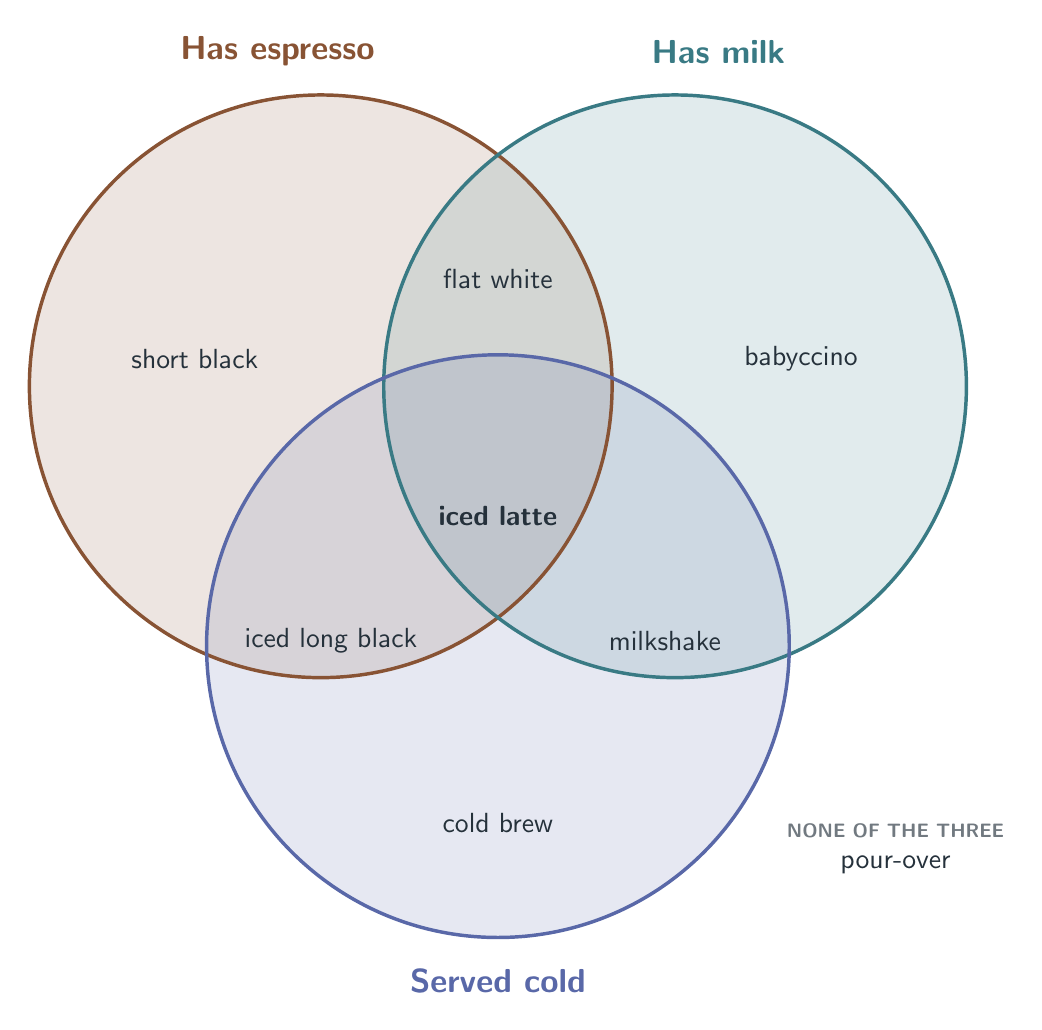
\begin{tikzpicture}[font=\sffamily, every node/.style={text=ink}]
  % Three translucent sets; the intersections retain the outlines of every set.
  \fill[espresso,opacity=.15] (-2.25,1.3) circle (3.7);
  \fill[milk,opacity=.15] (2.25,1.3) circle (3.7);
  \fill[cold,opacity=.15] (0,-2) circle (3.7);
  \draw[espresso,line width=1.25pt] (-2.25,1.3) circle (3.7);
  \draw[milk,line width=1.25pt] (2.25,1.3) circle (3.7);
  \draw[cold,line width=1.25pt] (0,-2) circle (3.7);

  % Set labels sit just outside their respective circles.
  \node[font=\sffamily\bfseries\large, text=espresso] at (-2.8,5.55) {Has espresso};
  \node[font=\sffamily\bfseries\large, text=milk] at (2.8,5.55) {Has milk};
  \node[font=\sffamily\bfseries\large, text=cold] at (0,-6.25) {Served cold};

  \tikzset{drink/.style={font=\sffamily\normalsize,align=center}}
  \node[drink] at (-3.85,1.65) {short black};
  \node[drink] at (3.85,1.65) {babyccino};
  \node[drink] at (0,2.67) {flat white};
  \node[drink] at (-2.12,-1.93) {iced long black};
  \node[drink] at (2.12,-1.93) {milkshake};
  \node[drink,font=\sffamily\bfseries] at (0,-.35) {iced latte};
  \node[drink] at (0,-4.25) {cold brew};

  % A drink outside every circle is explicitly in the complement.
  \node[font=\sffamily\scriptsize\bfseries, text=ink!65] at (5.05,-4.35) {NONE OF THE THREE};
  \node[drink] at (5.05,-4.78) {pour-over};
\end{tikzpicture}
\end{document}
